% sequential circuit computing the sum of eight numbers
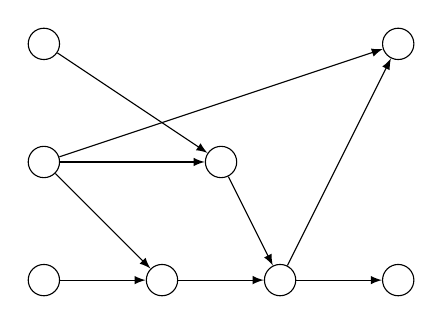
\begin{tikzpicture}
    [
        vertex/.style={circle, scale=1.2, draw,},
        edge/.style={-latex,},
        scale=1.5,
    ]

    % sequential dag
    \node (1) at (0,0)    [vertex] {};
    \node (2) at (0,1)    [vertex] {};
    \node (3) at (0,2)    [vertex] {};
    \node (4) at (1,0)    [vertex] {};
    \node (5) at (1.5,1)    [vertex] {};
    \node (6) at (2,0)    [vertex] {};
    \node (7) at (3,0)    [vertex] {};
    \node (8) at (3,2)    [vertex] {};

    \draw [edge] (1) -- (4);
    \draw [edge] (2) -- (4);
    \draw [edge] (2) -- (5);
    \draw [edge] (2) -- (8);
    \draw [edge] (3) -- (5);
    \draw [edge] (4) -- (6);
    \draw [edge] (5) -- (6);
    \draw [edge] (6) -- (7);
    \draw [edge] (6) -- (8);

\end{tikzpicture}         
